\chapter{Grundlagen}\label{chapter:basics}
In diesem Kapitel sollen die Grundlagen, die in dieser Arbeit benötigt werden, besprochen werden und bildet den Theorieteil der Thesis. Zuerst wird auf die mathematischen Grundlagen eingegangen, die zum Definieren von Verlustfunktionen für generative Machine-Learning-Modelle essentiell sind. Ziel dieses Teils ist es die Frage zu beantworten, wie weit eine Wahrscheinlichkeitsverteilung von einer anderen entfernt ist, um die Distanz anschließend zu minimieren. Das Minimieren der Entfernung zwischen Verteilungen wird in darauf folgenden Abschnitten verwendet, um Generative-Adversarial-Networks zu trainieren.

Neben den mathematischen Grundlagen werden einige grundlegende Bausteine für die
Entwicklung von hochqualitativen Feature-Extraktoren für die Objekterkennung auf
mobilen Endgeräten erläutert. Diese werden in späteren Kapiteln verwendet, um
neue neuronale Netzwerke zu entwickeln, die unter anderem menschliche Posen aus
Bildern sehr genau extrahieren und letztlich Bewegungen erkennen können. Hierfür
ist eine hohe Semantik bei einer hohen Qualität bzw. Auflösung unabdingbar, um
auch kleine Merkmale wie Hände erkennen zu können. Deshalb werden
Feature-Pyramid-Networks (FPNs) erläutert, die mithilfe eines sogenannten
Backbones hochauflösende Features mit einer hohen Semantik extrahieren können
während einfache Faltungsschichten (Convolutional-Layer) zwar ein hohes
Verständnis entwickeln, jedoch eine kleine Auflösung dieser Features besitzen.

Neben den FPNs soll auch die Idee hinter Residual-Neural-Networks (ResNets) erläutert werden.

\section{Notationen}
In dieser Arbeit werden verschiedene Notationen aus der Statistik und dem
Machine-Learning-Umfeld verwendet und sollen hier aufgrund der Les- und
Verständlichkeit aufgelistet werden.

\paragraph{Erwartungswert.}
Der Term $\mathbb{E}_{x \sim P}\left[f(x)\right]$ stellt den Erwartungswert
einer Verteilung $P$ dar und liest sich als \textit{erwarteter Wert von
$f(x)$ unter $x$ verteilt als $P$}.

\paragraph{Berechnung von Gradienten.}
Der Term $\nabla_w\left[f(x)\right]$ stellt die Berechnung der Gradienten von
den Parametern $w$ mithilfe der Loss-Funktion $f$ dar.

\paragraph{Euklidische Norm.}
Der Term $\| v \|$ stellt die euklidische Norm von $v$ dar. Sie ist definiert als die Summer aller Quadrate der Komponenten von $v$, also $\| v \| = \| v \|_2 = \sqrt{v_1^2 + v_2^2 + ... + v_n^2}$.

\section{Lipschitzstetigkeit}
\begin{definition}[K-Lipschitzstetigkeit]
Seien $(X, d_X)$ und $(Y, d_Y)$ metrische Räume. Eine Abbildung $f: X \to Y$
wird als K-lipschitzstetig bezeichnet, wenn
\[
    d_Y(f(x_1), f(x_2)) \leq K \cdot d_X(x_1, x_2)
\]
für alle $x_1, x_2 \in X$ gilt. $K$ wird hierbei als Lipschitzkonstante
bezeichnet und muss immer $K \geq 0$ erfüllen.
\end{definition}

\section{Kullback-Leibler-Divergenz}
Die Kullback-Leibler-Divergenz (KL-Divergenz) misst, wie sehr sich zwei
Verteilungen voneinander unterscheiden und hat seinen Ursprung in der
Informationstheorie. 
\begin{definition}[Kullback-Leibler-Divergenz \cite{arjovsky2017wasserstein}]
Seien $P$ und $Q$ zwei Wahrscheinlichkeitsfunktionen über den gleichen
Wahrscheinlichkeitsraum $X$. Dann ist der Abstand bzw. die Divergenz der
beiden Verteilungen definiert als
\[
    D_{KL}(P \lvert\lvert Q) = \sum_{x \in X} P(x) \log \frac{P(x)}{Q(x)}.
\]
\end{definition}
Dabei gibt $P \lvert\lvert Q$ eine Divergenz von der Ausgangsverteilung $P$
zur Zielverteilung $Q$ an. Das Messen der Divergenz zwischen zwei
Wahrscheinlichkeitsverteilungen findet insbesondere im Machine-Learning statt,
um künstliche neuronale Netze und ihre Gewichte zu trainieren. Deshalb kann
die KL-Divergenz auch als Loss-Funktion verwendet werden. Bemerkenswert ist
hierbei, dass die KL-Divergenz asymmetrisch ist, also $D_{KL}(P \lvert\lvert
Q) \neq D_{KL}(Q \lvert\lvert P)$. Die Distanz zwischen zwei Verteilungen
unterscheidet sich demnach je nach Ausgangsverteilung.

\section{Jensen-Shannon-Divergenz}
\begin{definition}[Jensen-Shannon-Divergenz \cite{arjovsky2017wasserstein}]
Seien $P$ und $Q$ zwei Wahr\-schein\-lichkeitsfunktionen über den gleichen
Wahrscheinlichkeitsraum $X$. Dann ist die Jensen-Shannon-Divergenz der
beiden Verteilungen definiert als
\[
    D_{JS}(P \lvert\lvert Q) = \frac{1}{2} D_{KL}(P \lvert\lvert M) + \frac{1}{2} D_{KL}(Q \lvert\lvert M) \quad\quad \text{mit} \;\; M = \frac{1}{2}(P + Q)
\]
\end{definition}
Die Jensen-Shannon-Divergenz kann als Erweiterung der
Kullback-Leibler-Divergenz angesehen werden. Im Gegensatz zur
Kullback-Leibler-Divergenz ist die Jensen-Shannon-Divergenz (JS-Divergenz)
symmetrisch. Das bedeutet, dass der Abstand zwischen zwei
Wahrscheinlichkeitsverteilungen gleich groß ist, egal von welchen er beiden
Distributionen aus betrachtet wird.

\section{Wasserstein-Abstand}
Eine weitere Methode zum Messen des Abstands zwischen zwei
Wahrscheinlichkeitsverteilungen ist die Berechnung des Wasserstein-Abstands.

\begin{definition}[Wasserstein-Abstand \cite{arjovsky2017wasserstein}]
Seien $P_r$ und $P_g$ zwei Wahrscheinlichkeitsverteilungen, dann ist der
Wasserstein-Abstand definiert als
\[
    W(P_r, P_g) = \inf_{\gamma \in \Pi(P_r, P_g)} \mathbb{E}_{(x, y) \sim \gamma} \left[\|x - y\|\right],
\]
wobei $\Pi(P_r, P_g)$ die Menge aller gemeinsamen Verteilungen $\gamma(x,
y)$ darstellt, dessen Grenzen $P_r$ und $P_g$ sind.
\end{definition}

Der Term $\gamma(x, y)$ stellt dabei die \textit{Masse} dar, die von $x$ nach
$y$ transportiert wird, um schließlich die Verteilung $P_r$ in die Verteilung
$P_g$ umzuformen. Aus diesem Grund ist der Wasserstein-Abstand auch als
\textit{Earth-Mover-Abstand} (EM-Abstand) bekannt.

\section{Residual-Neural-Networks}
Mit \cite{he2015deep} wurde ein neues Framework zum Trainieren von tiefen
neuronalen Netzen vorgestellt. Ein großes Problem mit sehr tiefen neuronalen
Netzen ist, dass diese zu einem größeren Fehler im Training führen. Dies führt
ebenfalls zu einem erhöhten Test-Fehler. Diese Fehler werden überraschenderweise
immer größer, je tiefer das Netzwerk ist und das Phänomen wird als
\textit{Degradation} bezeichnet. Dies ist auch bei der Genauigkeit solcher Netze
beobachtbar. Ist die Genauigkeit gesättigt und erhöht man nun die Tiefe des
Netzes, so degradiert die Genauigkeit schnell. Laut \cite{he2015deep} liegt dies
nicht am Overfitting (Überanpassung). Overfitting beschreibt die
Überspezialisierung eines Machine-Learning-Modells, welches sich zu sehr an den
dahinterliegenden Datensatz angepasst hat. Ein solches Modell kann nicht mehr
zuverlässig mit Daten außerhalb des zum Trainieren verwendeten Datensatzes
betrieben werden. Anders ausgedrückt besitzt das Netzwerk eine sehr hohe
Genauigkeit beim Arbeiten mit dem Trainingsdatensatz, aber eine signifikant
niedrigere Genauigkeit beim Arbeiten mit dem Testdatensatz.

Abhilfe für Degradation sollen die Residual-Networks (ResNets) mithilfe von
\textit{Building-Blocks} schaffen. Anstatt die Abbildung
$F(x)$ bei normalen gestapelten Schichten zu optimieren, wird bei ResNet das
Residuum $F(x) + x$ modelliert. Dies kann mithilfe von Shortcut-Connections
(Abkürzungsverbindungen) realisiert werden (siehe Abbildung
\ref{fig:resnet-building-block}).

\begin{figure}
    \centering
    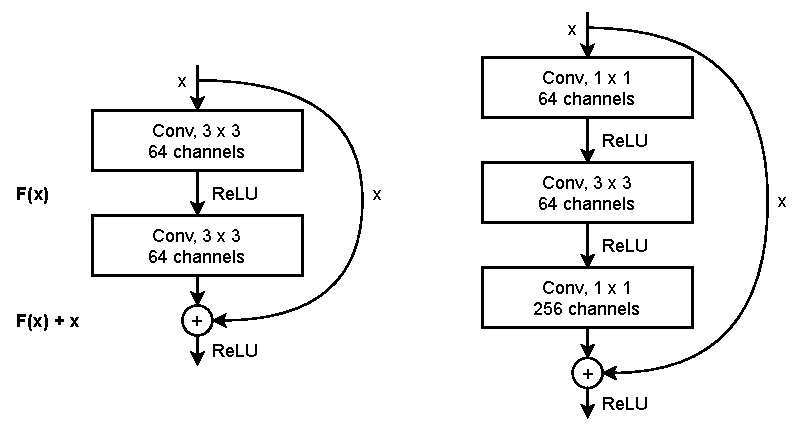
\includegraphics[width=0.8\textwidth]{images/resnet_building_block.pdf}
    \caption{Schemata für Building-Blocks eines ResNets \cite{he2015deep}. Die
    Shortcut-Connection ist die Identität von dem Eingabeparameter $x$. Links ist ein einfacher Residual-Block dargestellt während rechts ein tieferer, soganannter Bottleneck-Block dargestellt wird.}
    \label{fig:resnet-building-block}
\end{figure}

Abhängig von den Anforderungen können nun entsprechend tiefe Netze eingesetzt
werden, indem die Building-Blocks gestapelt eingesetzt werden. In
\cite{he2015deep} werden außerdem ein paar Architekturen vorgestellt, die
erfolgreich auf den ImageNet-Datensatz \cite{deng2009imagenet} evaluiert wurden.
Diese unterscheiden sich hauptsächlich in der Anzahl der verwendeten Schichten
und sind in Tabelle \ref{table:resnets} zu sehen. Jeder dieser Residual-Blocks,
egal ob einfacher Building- oder Bottleneck-Block, kann einen Stride besitzen.
Dabei ist wichtig, dass der entsprechende Stride nur auf die erste
Faltungsschicht des gesamten Blocks angewandt wird. Die restlichen Schichten
besitzen demnach immer einen Stride von 1. Die Ergebnisse nach dem Trainieren
dieser Netze haben gezeigt, dass das Degradation-Problem gelöst werden konnte,
sodass tiefere Netze mithilfe von Residual-Blocks auch einen geringeren Fehler
erzeugen, also genauer arbeiten als weniger tiefe Netze.

\begin{table}
    \scriptsize
    \begin{tabularx}{\textwidth}{X|X|c|c|c|c|c}
        \hline
        layer name & output size & 18-layer & 34-layer & 50-layer & 101-layer & 152-layer \\ \hline
        conv1 & $112 \times 112$ & \multicolumn{5}{c}{$7 \times 7$, 64, stride 2} \\ \hline
        \multirow{2}{*}{conv2\_x} & \multirow{2}{*}{$56 \times 56$} & \multicolumn{5}{c}{$3 \times 3$, max pool, stride 2} \\ \cline{3-7}
        & & \resnetblocksimple{64}{64}{2} & \resnetblocksimple{64}{64}{3} & \resnetbottleneck{64}{256}{3} & \resnetbottleneck{64}{256}{3} & \resnetbottleneck{64}{256}{3} \\ \hline
        conv3\_x & $28 \times 28$ & \resnetblocksimple{128}{128}{2} & \resnetblocksimple{128}{128}{4} & \resnetbottleneck{128}{512}{4} & \resnetbottleneck{128}{512}{4} & \resnetbottleneck{128}{512}{8} \\ \hline
        conv4\_x & $14 \times 14$ & \resnetblocksimple{256}{256}{2} & \resnetblocksimple{256}{256}{6} & \resnetbottleneck{256}{1024}{6} & \resnetbottleneck{256}{1024}{23} & \resnetbottleneck{256}{1024}{36} \\ \hline
        conv5\_x & $7 \times 7$ & \resnetblocksimple{512}{512}{2} & \resnetblocksimple{512}{512}{3} & \resnetbottleneck{512}{2048}{3} & \resnetbottleneck{512}{2048}{3} & \resnetbottleneck{512}{2048}{3} \\ \hline
        & $1 \times 1$ & \multicolumn{5}{c}{average pool, 1000-d fc, softmax} \\ \hline
        \multicolumn{2}{c|}{FLOPs} & \num{1.8e9} & \num{3.6e9} & \num{3.8e9} & \num{7.6e9} & \num{11.3e9} \\ \hline
    \end{tabularx}
    \caption{Architekturen für ImageNet \cite{he2015deep}. Es werden die gestapelten Schichten bzw. Building-Blocks für ResNet-18, -34, -50, -101 und -152 aufgelistet. Die Building-Blocks werden hier als Matrix dargestellt und geben pro Zeile die Kernelgröße und Anzahl der Kanäle der Faltungsschichten an. Das Multiplikationszeichen hinter den Matrizen gibt die Anzahl der verketteten Building-Blocks an.}
    \label{table:resnets}
\end{table}

\section{Feature-Pyramid-Networks}
Bei der Objekterkennung ist beim Erlernen der Features eines Bildes die
Auflösung dieser Features sehr gering. Feature-Pyramid-Networks (FPN) haben die
Aufgabe, eine hohe Semantik bei einer hohen Auflösung zu generieren. Häufig sind
diese Netzwerke nur Teil eines Backbones bzw. werden dahinter geschaltet. Als
Backbone-Modell kann zum Beispiel AlexNet, MobileNet und ResNet dienen. In
Kombination mit einem FPN werden diese Netze damit zu einem Feature-Extractor
umgewandelt, der eine hohe Semantik bei einer hohen Auflösung der Features
erlernen kann. Der Weg von der Eingabe über das Backbone-Modell wird auch als
\textit{Bottom-Up-Pathway} bezeichnet, während der Weg vom Backbone über die
Feature-Pyramid als \textit{Top-Down-Pathway} bezeichnet wird
\cite{lin2017feature}.

Anfänglich wurden FPNs in Verbindung mit ResNet-Backbones eingeführt (siehe
Abbildung \ref{fig:resnet-fpn}). Die Eingabe ist ein $224 \times 224 \times 3$
Bild und wird mithilfe der ersten ResNet-Schicht (C1) in $112 \times 112 \times
64$ Filter mithilfe eines Convolutional-Layers mit einem Stride von 2 und einem
$7 \times 7$ Kernel umgeformt. Anschließend wird die Ausgabe in ein
Max-Pooling-Block gegeben, welcher die Eingabe in $56 \times 56 \times 128$
Filter umwandelt. Die nächsten Blöcke sind für die Einbettung von FPNs am
wichtigsten. Der folgende Block (C2) besteht aus mehreren Residual-Blocks,
welche zusammen einen Stride von 1 ergeben und 256 Filter erzeugen. Diese Blöcke
werden zusammengefasst auch \textit{Bottlenecks} genannt. Darauf folgen drei
weitere Bottleneck-Blöcke (C3, C4, C5) mit einem Stride von 2. Nach C5 ensteht
somit eine Ausgabe von $7 \times 7 \times 2048$. Soweit zum Aufbau des
Bottom-Up-Pathways. Der Top-Down-Pathway wird mithilfe von Verbindungsschichten
(Laterals) mit dem Backbone verbunden. Diese haben die Aufgabe, die Anzahl der
Filter aus dem Bottom-Up-Pathway so umzuformen bzw. anzugleichen, sodass diese
im Top-Down-Pathway miteinander addiert werden können. Hierfür werden
Convolutional-Layer mit einem $1 \times 1$ Kernel und 256 Filtern verwendet,
sodass lediglich die Anzahl der Filter transformiert werden. Im Konkreten
bedeutet dies, dass die Ausgabe von C5 von $7 \times 7 \times 2048$ auf die Form
$7 \times 7 \times 256$ gebracht wird.  Die Größe dieser Ausgabe wird nun
mithilfe von Upsampling (M5) verdoppelt und mit der Ausgabe der
Lateralverbindung von C4 addiert (M4). Dies wird mit den übrigen
Lateralverbindungen und Bottleneck-Blöcken verkettet wiederholt, sodass das FPN
schließlich vier Ausgaben mit den Größen $56 \times 56 \times 256$, $28 \times
28 \times 256$, $14 \times 14 \times 256$ und $7 \times 7 \times 256$ (M5, M4,
M3, M2) ausgibt. Betrachtet man nun die letzte Ausgabe M5 relativ zum
Eingabeformat, so besitzt diese Architektur einen Stride von 4. Das Problem beim
Vergrößern der Filter ist, dass dabei ein Alias-Effekt auftritt, das Bild also
verschwommen wirkt. Hierfür dienen Smoothing-Layer, welche wiederum nichts
weiter als Convolutional-Layer mit einem $3 \times 3$ Kernel und einem Stride
von 1 sind. Entsprechend werden die Ausgaben M5 - M2 verschärft und ergeben
Features mit einer hohen Auflösung und einer hohen Semantik, die nun wahlweise
für die Objekterkennung verwendet werden können.

\begin{figure}
    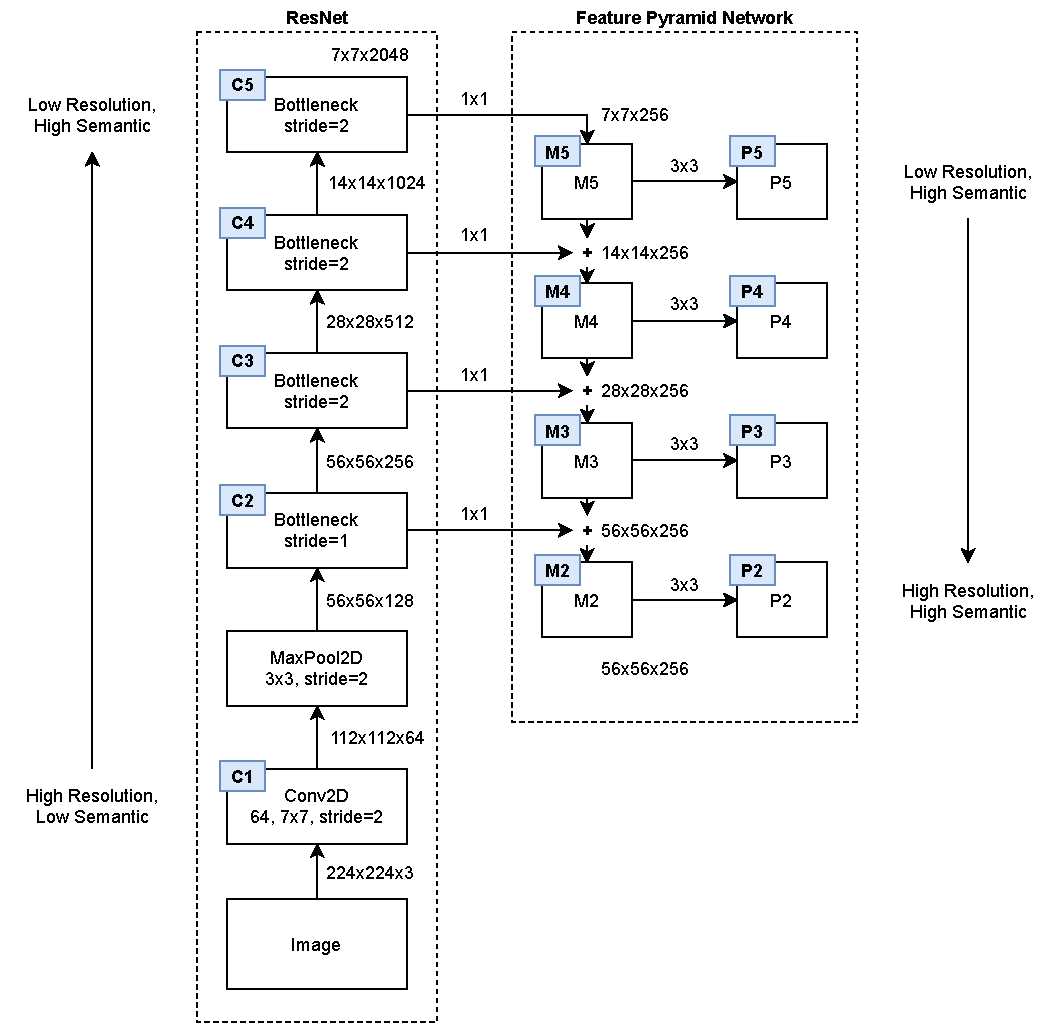
\includegraphics[width=\textwidth]{images/ResNet_FPN.pdf}
    \caption{Architektur eines Feature-Extractors als Feature-Pyramid-Network
    mit ResNet als Backbone.}
    \label{fig:resnet-fpn}
\end{figure}
